%%%%%%%%%%%%%%%%%%%%%%%%%%%%%%%%%%%%%%%%%%%%%%%%%%%%%%%%%%%%%%%%%%% 
%                                                                 %
%                            CHAPTER FOUR                          %
%                                                                 %
%%%%%%%%%%%%%%%%%%%%%%%%%%%%%%%%%%%%%%%%%%%%%%%%%%%%%%%%%%%%%%%%%%% 

% EXPERIMENT COMMANDS
% ibeis -e rank_cdf --db humpbacks_fb -a default:has_any=hasnotch,mingt=2 -t default:proot=BC_DTW,decision=max,crop_dim_size=750,crop_enabled=True,manual_extract=True,use_te_scorer=True,ignore_notch=False,te_net=annot_res,te_score_method=avg,equalize_hist=False,kp_net=256_decoupled,tol=10 --dpath=/home/zach/data/results --save=<etc>.png --clipwhite

\chapter{Results} \label{sec:results}

In this chapter we present the results that this method achieves on the Flukebook dataset.
The main results for the optimal method are given briefly, and then we discuss how different variations on the method affect accuracy.

\section{Main method}

%TODO: Figure out optimal method, put results here

\subsection{Characterization of Success cases}

\subsection{Characterization of Failure cases}

\section{Variations}

\subsection{Keypoint Extraction}

\subsubsection{Keypoint Extractor}

In this section, we detail the training results of the fluke keypoint extractor, and note issues with it.
We also show the variation in accuracy between keypoint extractors run on different sized inputs.

\subsubsection{Manual versus Automatic}

One interesting note is to see how the final keypoint extractor compares with the manual annotations provided for the dataset.
In Figure (TODO), we can see that when using manual annotations, we get a slight boost in accuracy using the notch as a control point.
However, when the keypoint extractor network takes over, the inaccuracies in the notch prediction produce worse trailing edge artifacts than inaccuracies in the left / right tips --- so it's better to ignore it.

It must be stated that some of these manual annotations made it into the keypoint extractor's training set, however the vast majority of its training set comes from an external dataset.
Additionally, we can see from its training results that the keypoint extractor generalizes well regardless.

\subsubsection{Varying training image sizes}

Intuitively, the bigger the image the better the prediction can be, but at the expense of requiring more parameters to handle the input.
The primary difference between the networks that were trained to handle different size inputs is that, in order to ensure that all inputs to the final dense layers have the same spatial size ($2\times2$) across the different networks, an extra convolutional and pooling layer is added.

As seen in Figure (TOD), resizing all images to $256 \times 256$ achieves the highest accuracy.

% TODO Put in vary_kp_size.png

\subsubsection{STN} % Maybe?

We also briefly experimented with an Spatial Transformer Network.
This was largely motivated by the tendency of the keypoint extractor to do a terrible job of predicting fluke keypoints on flukes that did not 'fill' the image horizontally.
Unfortunately, we could not get the STN to converge at a better accuracy than the standard keypoint extractor, even if we held its parameters fixed for a few training epochs.
Usually, the STN would produce nonsensical transformations of the image.

% TODO: Figure showing this

\subsection{Image Preprocessing}

In this part we also detail some simple image preprocessing steps that we took (given the fluke keypoints) that greatly influenced the efficacy of the method.
Ultimately we just ended up using a combination of cropping and resizing the image so as to normalize the length of the trailing edge, as detailed below.

We also note that we originally tried histogram equalization as part of the preprocessing pipeline, althoough it produced significantly worse trailing edges (and subsequently matching accuracy).

\subsubsection{Cropping and Image Width}

While, with dynamic time warping, we theoretically can match sequences of similar or different lengths, the distances are distorted by large differences in actual trailing edge length.
Since we are only interested in the width of an image (assuming that the trailing edge is roughly horizontal in the image), we can get every trailing edge to have exactly some fixed length $w$ by the following process

\begin{itemize}
    \item Crop the image horizontally between the left and right columns found by the keypoint extraction process (or manually determined).
    \item Resize the cropped image to some fixed width $w$ while preserving the aspect ratio, using Lanczos interpolation. % TODO find citation for this
\end{itemize}

In this way, we standardize the trailing edge length so that image scale does not affect detection accuracy too much.

% TODO figure comparing crop and no crop no resize
One major caveat with this process is of course that using the keypoint extractor's predictions can cause catastrophic failures in this process (e.g. the left and right points are nowhere near a fluke), however in practice we found that it works well enough -- far better than the alternative.

\paragraph{Trailing Edge Length}

Determining what $w$ should be is not super obvious.
Ideally, one would simply look at the mode or average post-crop width, and try to keep $w$ around there.

We can see in Figure (TODO vary\_crop\_size.png) that the optimal post-crop $w$ for this dataset (of the few we evaluated) is 750 pixels.
Figure (TODO te\_size\_hist\_fb.png) shows the histogram of post-crop widthsi showing that $750$ is a good width, which is what we use as a default.

Intuitively, this implies that the less the image has to be resized, the better the trailing edge.

\subsection{Trailing Edge Extraction}

There are a lot of variants on trailing edge scoring networks that were attempted, often with mixed results. 
One major result that we found was that, when using the averaging method to combine the trailing edge scores with $N_y$, having a robust trailing edge prediction wasn't as important as having a detailed trailing edge.

\subsubsection{Trailing Edge Scorer variations}

The various trailing edge scorer architectures and their results on the task they were trained for is detailed in the previous chapter --- here we show the actual matching accuracies that each one produced.

Overall, we were unable to get a significant improvement from any trailing edge scorer besides the 'Simple' all convolutional scorer.
We theorize that this is because it could correct some mistakes made by the gradient only method (although it made many of the same mistakes itself) while providing detailed trailing edges.

More importantly, it appears that blocky trailing edge scores (such as those produced by any of the networks that are required to upsample their predictions) result in blocky trailing edges, which result in lower quality matches. 

\subsubsection{Combining $N_y$ and $T_y$}

We only evaluate the 'average' method here, and show that the mixing parameter $\beta$ has a significant effect on matching accuracy.

In Table (TODO: generate cartesian product of score weights and scorers), we can see that simply a pixel-wise average of $N_y$ and $(1-T_y)$ (i.e. $\beta = 0.5$) produces the best results.

\subsubsection{Number of neighbors in the extraction}

The number of neighbors $n$ effectively limits the slope of the trailing edge.
We limit it to an odd number for convenience.
On the one hand, a lower $n$ can cause the trailing edge to be limited in vertical breadth, but does prevent it from going way off course.
Despite this, with trailing edge scoring in place, it might be beneficial to increase $n$ so as to avoid parts of the trailing edge that continually 'max out' the number of neighbors, i.e. parts of the trailing edge that require a higher slope than would be allowed.

Ultimately, we can see in Figure (TODO: vary\_neighbors.png) that limiting the number of neighbors to the immediate neighborhood (i.e. $n = 3$) produces a significant boost over a larger neighborhood.
While the trailing edges extracted with $n = 3$ can be somewhat less detailed, they are less likely to go completely off course.
We hypothesize that despite the trailing edges being less detailed, the extraction artifacts (e.g. significant sections of the trailing edge where the bottom or top neighbor is consistently chosen) are produced in a way that is unique to the trailing edge.

\subsection{Curvature Extraction}

Curvature extraction is one of the least parameterized part of the process, however figuring out what the optimal values of $S$ and its cardinality is non-trivial.
One major point is that increasing the cardinality of $S$ increases the time it takes to evaluate the dynamic time warping, and as such we try to keep it at a small value (i.e. $|S| = 4$).

\subsubsection{Different scales}

We can look at each scale as measuring the curvature of some percentage of the trailing edge around the given point.
Intuitively, since the meaningful differences in trailing edge can be fairly small, it makes sense to measure a small curvature scale.
Additionally, this gives the most diversity in the trailing edge, as larger curvatures will change less and less from one point to the next.

However, larger curvatures are also less sensitive to noise, and thus small trailing edge extraction failures.


\begin{figure*}[t]%
	\centering
	\subfloat[][]{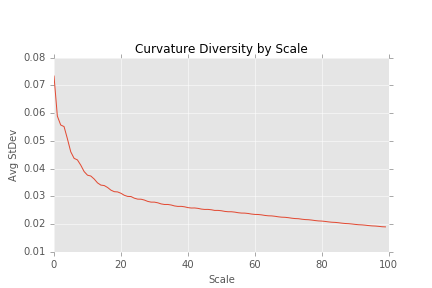
\includegraphics[width=0.5\textwidth]{../images/results/curvature_diversity_fb.png} }%
	\subfloat[][]{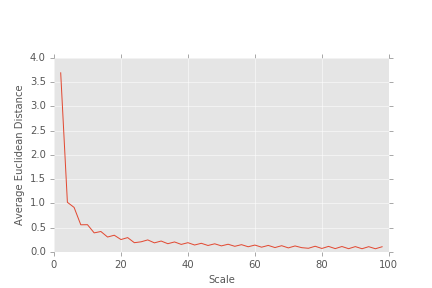
\includegraphics[width=0.5\textwidth]{../images/results/interscale_diff_fb.png} }%
	\caption[]{\textbf{Curvature Diversity}. Left panel (a) shows the average standard deviation of the (fixed length) curvature at different scales. Right panel (b) shows the average Euclidean distance between successive scales of curvature}
    	\label{fig:curvature_diversity}
\end{figure*}


We find that (as shown in the left panel of Figure \ref{fig:curvature_diversity}) as block curvature scale is increased, the diversity at any given point in the curvature (if it is of a fixed size) goes down drastically. 
As a result, we stick to the lower end of the scale, keeping the curvature scales measured below 15\%.

We can also see on the right side of Figure \ref{fig:curvature_diversity} that successive curvature scales show bigger differences at lower scales than at higher scales, which reinforces this need, but that it's advantageous to make bigger jumps between scales to maximize diversity while minimizing computation time.

Based on the above, we evaluate scales that run from 1\% to 15\%, with varying levels of resolution (TODO: set this up and run it).

\subsubsection{Number of scales}

Increasing the number of scales measured could potentially give more detail to work with, however at some point successive scales will not produce a meaningful difference from other scales, an effect that will become more notable the larger the scales get. % TODO: Figure this out based on the difference between successive curvature scales
Additionally, beyond some percentage of the trailing edge the curvature that is extracted becomes very uniform, and thus useless for matching. % TODO: Figure showing this

\subsection{Dynamic Time Warp Matching}

The main variants shown in this section are the different Sakoe-Chiba bound windows and the scale weighting term in the curvature distance function.

\subsubsection{Weighting the different scales}

There are many ways to produce the weights $s_w$ for curvatures, but intuitively there should be a monotonic relationship between curvature scale and importance.

We could specify this relationship as a ratio $W$ of importance between successive pairs of curvatures (increasing in size).
We parameterize that importance by giving each scale the weight $s_w = [W^i \forall i \in [0,|S|]$.
In order to maintain this ratio without blowing up the distances, we also normalize so that $\sum s_w = 1$.

Figure (TODO: vary\_weight\_import.png) shows that despite this effort, it appears that equally weighting each curvature scale provides the best performance.

\subsubsection{Window size}

In Figure (TODO: vary\_window\_size.png), we can see that if we decrease the window (i.e. the Sakoe-Chiba bound) size, at around 10\% of the query trailing edge length we maintain the same accuracy as the full window (i.e. 100\$), but below this accuracy is severely affected.
Thus, we use this value for the window size so as to minimize computation time while maintaining the total accuracy.

Additionally, while it's possible for gross mismatches to occur from there being no window boundary, we can see from Figure (TODO same as above) that this does pose a problem for this dataset.

\subsubsection{Aggregating over multiple trailing edges per identity}

Determining the identity of a given query image given distances to other images in the database is not entirely simple when there are multiple database images for a given individual.
Essentially we need to transform these distances from query image to database image into distances from query to known individual.
To do so we evaluate two options given a group of distances for an individual --- either the average distance or the minimum distance.

We find that the minimum distance version provides significantly better accuracy than the average distance. % TODO show this
While this is a bit surprising given that most of the individuals in the dataset only have two images associated, there are still a significant amount of individuals for whom there are more than that.
That said, the minimal distance version also is in line with the LNBNN decision criterion used by Hotspotter \cite{crall_hotspotter_2013}, and as such as theoretical backing. % TODO: lay out what this theoretical backing actually is

\section{In Combination with Hotspotter}

\subsection{Failure cases}

\subsection{Characterization of when to use which method}


%%% Local Variables: 
%%% mode: latex
%%% TeX-master: t
%%% End: 
